\documentclass[../../InformazioneQuantistica.tex]{subfiles}

\begin{document}

\section{Matrici densità - parte 2}
\lesson{6 \orangedot}{14/3/2019}

\subsection{Correlazioni tra stati}
Nella sezione precedente abbiamo notato che $\rho_{12}=\rho_1 \otimes \rho_2$ vale solo se $\rho_1$ e $\rho_2$ sono \textbf{indipendenti}, cioè \textbf{scorrelati}. Se così non è, come nella maggior parte dei casi, $\rho_1$ e $\rho_2$ codificano solo una parte delle informazioni del sistema composto $\rho_{12}$, dato che mancano i termini di \textit{interazione} tra i due sottosistemi, che effettivamente in tal caso non hanno una individualità ben definita.\\

Esaminiamo allora, nello specifico, cosa significhi \textbf{correlazione}.\\
Partiamo dal caso più semplice di due variabili casuali classiche $x_i$ e $y_i$ con opportune distribuzioni di probabilità. Supponiamo che $x_i$ e $y_i$ assumano valori binari $\{1,-1\}$, corrispondenti per esempio all'esito di una misura di una certa osservabile sui due sistemi.
 Possiamo campionare $N$ volte le due variabili costruendo due vettori $\vec{x}$ e $\vec{y}$:
\begin{align*}
\vec{x} &= \{1, -1, -1,-1, \dots, -1\}\\
\vec{y} &= \{-1, 1, +1, +1\dots, +1\}
\end{align*} 
$\vec{x}$ e $\vec{y}$ corrispondono, fisicamente, a misure ripetute di osservabili con risultati binari (sì/no) eseguite sui due sistemi.\\
Supponiamo che le $x_i$ e $y_i$ si distribuiscano simmetricamente attorno a $0$, e cioè abbiano media nulla:
\begin{align*}
\bar{x} = 0; \qquad \bar{y}=0
\end{align*}
Un modo per quantificare la \textbf{correlazione} tra le due è dato dal calcolare la media del prodotto:
\begin{align*}
\overline{x\,y} = \frac{1}{N}\sum_{i=1}^N x_i\,y_i
\end{align*}

Ci si potrebbe aspettare che, poiché $\bar{x}=0$ e $\bar{y}=0$, anche $\overline{x\,y}=0$. In realtà è vero solo se le due variabili sono \textit{indipendenti}. Se esiste una qualche relazione tra le due, per cui $y$ tende ad assumere valori che dipendono da quelli di $x$ (e viceversa), non è detto che i singoli prodotti $x_i y_i$ si distribuiscano ancora in modo simmetrico.\\

Per esempio:
\begin{itemize}
\item Se $x_i=y_i$, avremo $x_i\,y_i=1$ $\forall i$, e quindi $\overline{x\,y}=1$. $x$ e $y$ si dicono allora \textbf{completamente correlate}
\item Se $x_i=-y_i$ si ha $x_i\, y_i=-1$ $\forall i$, da cui $\overline{x\,y}=-1$, e $x$ e $y$ sono \textbf{completamente anticorrelate}
\item Se $x_i\, y_i$ si distribuiscono simmetricamente attorno a $0$, $\overline{x\, y}=0$ e le due variabili si dicono \textbf{scorrelate}.
\end{itemize}
Nel caso generale avremo una correlazione \textit{parziale}, che si valuta tramite il \textbf{coefficiente di Pearson}\marginpar{Coefficiente di Pearson}\index{Coefficiente di Pearson}:
\begin{align*}
\sigma_{xy} = \frac{E[(x-\mu_x)(y-\mu_y)]}{\sigma_x \sigma_y} \qquad \begin{cases}
\mu_x = \bar{x}\\
\mu_y = \bar{y}
\end{cases}
\begin{cases}
\sigma_x^2 = \overline{(x-\mu_x)^2}\\
\sigma_y^2 = \overline{(y-\mu_y)^2}
\end{cases}
\end{align*}
dove $E(x)$ indica il valore di aspettazione (speranza matematica) di una certa variabile casuale $x$.\\
Notiamo che il coefficiente di Pearson corrisponde alla media di \textit{infiniti} prodotti $(x_i-\mu_x)\,(y_i-\mu_y)$ (per cui le $x_i$ e $y_i$ possono non essere simmetriche attorno a $0$), normalizzata alle loro dispersioni attorno alle loro medie.\\

Tale formula si adatta immediatamente al caso quantistico, calcolando medie di operatori:
\begin{align*}
E[(X-\mu_x)(Y-\mu_y)] &= \langle (\hat{X}-\langle \hat{X}\rangle)(\hat{Y}-\langle \hat{Y}\rangle)\rangle = \\
&= \avg{\hat{X}\hat{Y}} - \avg{\avg {\hat{X}}\hat{Y}} - \avg{\hat{Y}\avg{ \hat{X}}}+ \avg{\avg{\hat{X}}\avg{\hat{Y}}} = \\
&= \langle \hat{X}\hat{Y}\rangle -\cancel{ \langle \hat{X}\rangle \langle \hat{Y}\rangle} - \langle \hat{Y}\rangle \avg{\hat{X}} +\cancel{ \avg{\hat{X}}\avg{\hat{Y}}} =\avg{\hat{X}\hat{Y}}-\avg{\hat{X}}\avg{\hat{Y}}
\end{align*}

\subsection{Correlazioni ed entanglement}
La presenza di correlazioni è propria degli \textbf{stati} \textbf{entangled}, ossia stati composti non decomponibili in un prodotto tensore:
\begin{align*}
\ket{\phi} \neq \ket{\phi_1}\otimes \ket{\phi_2}
\end{align*}

Mostriamo infatti che \textbf{non} vi sono \textbf{correlazioni} tra le componenti di un sistema\marginpar{Stati non entangled non presentano correlazioni} \textbf{separabile}. Consideriamo uno stato $\ket{\psi}$ \textbf{non entangled} di un sistema composto $S$, per cui quindi vale:
\begin{align*}
\ket{\psi}=\ket{\psi_A}\otimes \ket{\psi_B}
\end{align*}
Siano $\hat{X}_A$ e $\hat{X}_B$ due generiche osservabili relative, rispettivamente, ai sottosistemi $A$ e $B$ che compongono $S$. Calcoliamone la correlazione $\sigma_{xy}$ a partire dalla definizione:
\begin{align*}
\sigma_{xy} &= \avg{\hat{X}_A \hat{Y}_B} - \avg{\hat{X}_A} \avg{\hat{Y}_B} = \\
&=\bra{\psi_A \psi_B} \hat{X}_A \hat{X}_B \ket{\psi_A \psi_B}- \bra{\psi_A \psi_B}\hat{X}_A \ket{\psi_A\psi_B}\bra{\psi_A\psi_B}\hat{Y}_B \ket{\psi_A\psi_B} =\\
&=\bra{\psi_A}\hat{X}_A \ket{\psi_A}\bra{\psi_B}\hat{X}_B \ket{\psi_B} - \bra{\psi_A}\hat{X}_A\ket{\psi_A}\bra{\psi_B}\hat{Y}_B\ket{\psi_B} = 0
\end{align*}

D'altro canto, per uno stato $\ket{\phi}$ non separabile (entangled), in generale $\sigma_{xy}$ può assumere valori non nulli: si hanno quindi \textbf{correlazioni} tra misure di osservabili eseguite sulle \textbf{diverse componenti} del sistema composto.

\subsection{Schmidt decomposition}
Come possiamo riconoscere uno stato \textbf{entangled}?\\
Per esempio, dato un sistema $S$ composto di due qubit $A$ e $B$, con $\hs_S = \hs_A \otimes \hs_B$, si nota immediatamente che:
\begin{align}\nonumber
\ket{\psi_1} &= \ket{0}_A\ket{0}_B
\intertext{è uno stato non correlato, mentre}
\ket{\psi_2} &= \frac{1}{\sqrt{2}}(\ket{0}_A \ket{1}_B + \ket{1}_A\ket{0}_B)
\label{eqn:bell-entangled}
\end{align}
è entangled (infatti è uno stato di Bell).\\
Tuttavia uno stato come:
\begin{align*}
\ket{\psi_3} = \frac{1}{\sqrt{2}}(\ket{0}_A\ket{1}_B + \ket{0}_A\ket{0}_B)
\end{align*}
\textbf{non} è entangled, dato che lo si può fattorizzare come:
\begin{align}
\ket{\psi_3} = \ket{0}_A \otimes \frac{1}{\sqrt{2}}(\ket{0}_B+\ket{1}_B)
\label{eqn:stato-fattorizzato}
\end{align}
In questo caso semplice (due soli fattori) la decomposizione si trova abbastanza in fretta, ma considerando più termini, oppure basi differenti da quella computazionale, il problema diviene sempre più complesso. Per esempio, il seguente stato $\ket{\psi_4}$ è entangled?
\begin{align*}
\ket{\psi_4} = \ket{0}_A \ket{0}_A - \ket{0}_A\ket{1}_B +\ket{0}_A\ket{1}_B  - \ket{1}_A\ket{1}_B
\end{align*}

Per rispondere a domande del genere conviene introdurre un risultato di algebra lineare, che permette di riscrivere un generico stato in una \q{forma minima}, dove stati fattorizzati sono scritti come un unico prodotto (come in \ref{eqn:stato-fattorizzato}), mentre gli stati entangled sono dati dalla somma di più prodotti (\ref{eqn:bell-entangled}), per cui la distinzione tra i due casi risulta evidente.\\

Tale processo prende il nome di \textbf{decomposizione di Schmidt}.\marginpar{Decomposizione di Schmidt}\index{Decomposizione di Schmidt} Consideriamo un'autofunzione $\ket{\psi}$ in uno spazio di Hilbert (separabile) di un sistema composto \textbf{bipartito}\footnote{Non è necessario che $A$ e $B$ siano singoli qubit. Per esempio potremmo considerare un sistema di $5$ qubit, separato in parte $A$ data dai primi $3$ e parte $B$ con i restanti $2$, e applicare lo stesso i risultati del teorema.}:
\begin{align*}
\ket{\psi}\in \hs = \hs_A \otimes \hs_B
\end{align*}
Allora esistono due \textbf{basi} ON $\{\ket{u_i}_A\}_{i=1}^{N_A}$ e $\{\ket{v_i}_B\}_{i'=1}^{N_B}$ per cui vale la decomposizione:
\begin{align}
\ket{\psi}=\sum_{i=1}^k \sqrt{p_i} \ket{u_i}_A \ket{v_i}_B \quad p_i \geq 0;\quad \sum_{i=1}^k p_i = 1; \quad k\leq\min\{\op{dim}\hs_A
, \op{dim}\hs_B\}\label{eqn:schmidt}
\end{align}

\textbf{Nota}: In (\ref{eqn:schmidt}) stiamo sommando sugli indici di una \textbf{sola} base. La decomposizione di Schmidt è quindi molto più semplice della normale decomposizione di $\ket{\psi}$ su due \textbf{generiche} basi $\{\ket{\alpha}_A\}$ e $\{\ket{\beta}_B\}$ di $\hs_A$ e $\hs_B$:
\begin{align}
\ket{\psi} = \sum_{ij} \gamma_{ij}\ket{\alpha_i}_A\ket{\beta_j}_B\label{eqn:decomp-composto}
\end{align}
dove la somma avviene su \textbf{entrambi} gli indici $i$ e $j$. Il risultato di Schmidt dimostra che è possibile \textit{rimuovere} uno dei due indici con una scelta opportuna delle due basi.\\

\textbf{Nota 2:} In informazione quantistica, si tende a far coincidere le basi $\{\ket{u_i}_A\}$ e $\{\ket{v_i}_B\}$ con opportune \textbf{basi computazionali} $\{\ket{i}_A\}, \{\ket{i'}_B\}$, in cui i ket sono denotati \q{in modo numerico} direttamente dall'indice $i$. In questa notazione la decomposizione di Schmidt diviene:
\begin{align*}
\ket{\psi}_{AB} =\sum_{i=1}^k \sqrt{p_i} \ket{i}_A \ket{i'}_B
\end{align*}
Per esempio, per $k=2$ avremo:
\begin{align*}
\ket{\psi}_{AB} = \sqrt{p_1}\ket{0}_A \ket{0'}_B + \sqrt{p_2}\ket{1}_A \ket{1'}_B
\end{align*}
dove gli apici mostrano che il qubit del sistema B può in generale utilizzare \q{livelli diversi} rispetto a quelli del qubit A (ossia in un'\textit{altra base}).\\

\textbf{Dimostrazione}.\marginpar{Dimostrazione}
Partiamo dalla scrittura (\ref{eqn:decomp-composto}) di $\ket{\psi}$ in due basi ON generiche $\{\ket{\alpha}_A\}$ e $\{\ket{\beta}_B\}$ di $\hs_A$ e $\hs_B$:
\begin{align}
\ket{\psi} = \sum_{ij}\gamma_{ij}\ket{\alpha_i}_A\ket{\beta_j}_B = \sum_i \ket{\alpha_i}_A \underbrace{\left( \sum_{j} \gamma_{ij} \ket{\beta}_B\right)}_{\ket{v_i}} = \sum_i \ket{\alpha_i}\ket{v_i}
\label{eqn:passo-decomp}
\end{align}
Il problema è che $\{\ket{v_i}\}$ \textbf{non} è, in generale, una base ON di $\hs_B$. Poiché i $\ket{v_i}$ dipendono dai fattori $\gamma_{ij}$, che a loro volta dipendono dalla scelta dei $\ket{\alpha_i}$, possiamo giocare su questi ultimi per avere la proprietà desiderata.\\
In effetti, si trova che se se invece di partire da una base ON $\{\ket{\alpha_i}\}$ generica per $\hs_A$, consideriamo la base $\{\ket{u_i}\}$ che \textit{diagonalizza} la matrice densità ridotta $\rho_1$, automaticamente $\{\ket{v_i}\}$ è ortogonale. Vediamo come.\\

Sia quindi $\{\ket{u}_i\}$ la base di $\hs_A$ in cui la matrice $\rho_1$ è diagonale:
\begin{align}
\rho_1 = \sum_i p_i\ket{u_i}_A \bra{u_i}_A
\label{eqn:rho-1-diagonal}
\end{align}
Dove $\rho_1$ è calcolata a partire dalla definizione:
\begin{align} \nonumber
\rho_1 &= \underset{2}{\op{Tr}}\rho_{12} =\underset{2}{\op{Tr}}\ket{\psi}\bra{\psi} \underset{(\ref{eqn:passo-decomp})}{=} \underset{2}{\op{Tr}} \left(\sum_{ij}\ket{\alpha_i}_A\ket{v_i}_B \bra{\alpha_j}_A\bra{v_j}_A \right) =\\ \nonumber
&\underset{(a)}{=} \sum_k \bra{k}_B \left(\sum_{ij}\ket{\alpha_i}_A\ket{v_i}_B \bra{\alpha_j}_A \bra{v_j}_B \right)\ket{k}_B =\\
&= \nonumber \sum_{ij} \ket{\alpha_i}_A\bra{\alpha_j}_A \left(\sum_k \braket{k|v_i} \braket{v_j|k}\right) =
 \sum_{ij} \ket{\alpha_i}_A\bra{\alpha_j}_A \left(\sum_k \bra{v_j}\underbrace{\ket{k}\bra{k}}_{\bb{I}}\ket{v_i}\right) =\\
&\underset{(b)}{=} \sum_{ij} \braket{v_j|v_i} \ket{\alpha_i}_A \bra{\alpha_j}_A
\label{eqn:rho-1-def}
\end{align}
dove in (a) usiamo una generica base ON $\{\ket{k}_B\}$ di $\hs_B$ per calcolare la traccia (che risulta la stessa per \textit{qualsiasi} scelta di base) e in (b) usiamo la completezza di Dirac per la base ON $\{\ket{k}_B\}$.\\
Usando allora la base $\{\ket{u_i}_A\}$ in (\ref{eqn:rho-1-def}), possiamo uguagliare con l'espressione equivalente in (\ref{eqn:rho-1-diagonal}), e giungere a:
\begin{align*}
\sum_{ij} \braket{v_j|v_i}\ket{u_i}_A \bra{u_i}_A = \sum_i p_i \ket{u_i}_A \bra{u_i}_A \Leftrightarrow \braket{v_j|v_i}=p_i\,\delta_{ij}
\end{align*}

\begin{align}
\ket{\psi}=\sum_{i, \alpha} c_{i\alpha}\ket{i}_A\ket{\alpha}_B = \sum_{i} \ket{i}_A \left(\sum_\alpha c_{i\alpha} \ket{\alpha}_B \right)\underset{(a)}{=} \sum_{i}\ket{i}_A \ket{\tilde{i}}_B
\label{eqn:psi-i-j}
\end{align}

Perciò si ha che, usando per $\hs_A$ la base $\{\ket{u_i}\}$ che diagonalizza $\rho_1$, la decomposizione (\ref{eqn:passo-decomp}) produce una base $\{v_i\}$ che è ortogonale. Perché sia orto\textbf{normale} basta normalizzare:
\begin{align*}
\ket{v_i}\mapsto \frac{1}{\sqrt{p_i}}\ket{v_i} \Rightarrow \braket{v_i|v_j}=\delta_{ij}
\end{align*}

E perciò la (\ref{eqn:passo-decomp}) porta alla tesi:
\begin{align*}
\ket{\psi} = \sum_i \sqrt{p_i} \ket{u_i}_A\ket{v_i}_B
\end{align*}

Vale inoltre (come mostrato nei passaggi intermedi):\marginpar{Matrici ridotte nelle basi di Schmidt}
\begin{align*}
\rho_1 = \underset{2}{\op{Tr}}\ket{\psi}\bra{\psi} = \sum_{i=1}^k
p_i \ket{u_i}\bra{u_i}
\end{align*}
E in maniera simmetrica si trova\footnote{Basta calcolare $\rho_{12} = \ket{\psi}\bra{\psi}$ usando per $\ket{\psi}$ il risultato della decomposizione di Schmidt, e quindi svolgere la traccia parziale.}:
\begin{align*}
\rho_2 = \underset{1}{\op{Tr}} \ket{\psi}\bra{\psi} = \sum_{j=1}^k p_{j} \ket{v_j}\bra{v_j}
\end{align*}
$k$ è il numero di coefficienti $p_i$ non nulli nell'espansione di $\ket{\psi}$ (pari al numero di \textbf{popolazioni} - cioè termini sulla diagonale - di $\rho_1$ o $\rho_2$). Per come è definita la sommatoria in (\ref{eqn:passo-decomp}), si ha che $k$ è al più pari al minimo tra la $\op{dim}\hs_A$ e $\op{dim}\hs_B$.\\
Usando le basi $\{\ket{u_i}_A\}$ e $\{\ket{v_i}_B\}$, perciò, $\rho_1$ e $\rho_2$ hanno la forma:
\begin{align*}
\rho_1 = \left(\begin{array}{ccccc}
p_1 & & & & \text{\huge0}  \\
 & \ddots &  & \text{\huge}&  \\
 & & p_k & & \\
 &\text{\huge} & & 0 &  \\
\text{\huge0} & \text{\huge} & & & \ddots
\end{array}
    \right)
    \qquad
\rho_2 = \left(\begin{array}{ccccc}
p_1 & & & & \text{\huge0}  \\
 & \ddots &  & \text{\huge}&  \\
 & & p_k & & \\
 &\text{\huge} & & 0 &  \\
\text{\huge0} & \text{\huge} & & & \ddots
\end{array}
    \right)
\end{align*}

\begin{expl}
\textbf{Dimostrazione alternativa}. Usando un teorema di algebra lineare, possiamo interpretare geometricamente la decomposizione in (\ref{eqn:passo-decomp}). Partiamo dalla decomposizione nelle basi ON generiche di $\hs_A$ e $\hs_B$:
\begin{align}
\ket{\psi}_{AB} =\sum_{i=1}^{\op{dim}\hs_A} \sum_{j=1}^{\op{dim}\hs_B} \gamma_{ij} \ket{\alpha_i}_A\ket{\beta_j}_B
\label{eqn:decomp-alternativa}
\end{align}
Interpretiamo i coefficienti $\gamma_{ij}$ come le entrate di una matrice $\Gamma$. Dall'algebra lineare si ha che è possibile scomporre ogni matrice $k \times k$ in un prodotto:
\begin{align*}
\Gamma = U \Lambda V
\end{align*}
dove $U$ è una matrice \textbf{unitaria} $d_A \times d_A$, $V$ è una matrice \textbf{unitaria} $d_B \times d_B$ e $\Lambda$ è una matrice $d_A \times d_B$ con $k$ numeri positivi $p_i > 0$ lungo la diagonale principale e $0$ altrimenti. Tale relazione prende il nome di \textbf{singular value decomposition}. Geometricamente, prendendo matrici reali, corrisponde al fatto che ogni trasformazione lineare può essere vista come una composizione di una rotazione $V$, un riscalamento $\Lambda$ e una rotazione finale $U$.\\

Dette $u_{ij}$ le entrate di $U$, e $v_{ij}$ quelle di $V$, i singoli elementi di $\Gamma$ derivano dal prodotto matriciale: 
\begin{align*}
\gamma_{ij} = \sum_{n=1}^k u_{in}\lambda_n v_{nj}
\end{align*}
Sostituendo tale risultato in (\ref{eqn:decomp-alternativa}) giungiamo a:
\begin{align*}
\ket{\psi}_{AB} = \sum_{n=1}^{k} \lambda_n\underbrace{ \left( \sum_{i=1}^{\op{dim}\hs_A} u_{in}\ket{\alpha_i}_A\right)}_{\ket{u_i}_A}\otimes\underbrace{ \left(\sum_{j=1}^{\op{dim}\hs_B} v_{nj}\ket{\beta_j}_B\right)}_{\ket{v_j}_B}
\end{align*}
Dato che $U$ e $V$ sono unitarie, esse trasformano basi ON in basi ON. Perciò $\{\ket{u_i}_A\}$ e $\{\ket{v_j}_B\}$ sono le basi ON di $\hs_A$ e $\hs_B$ che realizzano la decomposizione di Schmidt.
\end{expl}

\subsection{Schmidt Rank}
Consideriamo la decomposizione di Schmidt di uno stato $\ket{\psi}_{AB}$:
\begin{align*}
\ket{\psi}_{AB} = \sum_{i=1}^k \sqrt{p_i} \ket{u_i}_A \ket{v_i}_B
\end{align*}
Il numero $k$ di coefficienti $p_i > 0$ è detto \textbf{rango di Schmidt}, e consente di determinare se $\ket{\psi}$ è uno stato \textbf{entangled} o meno.\\

In particolare, vale:\marginpar{$k=1$ per stati non entangled}
\begin{align*}
k=1 \Leftrightarrow \ket{\psi} \text{ \textbf{non entangled }(separabile)}
\end{align*}
\textbf{Dimostrazione}.
Per $k=1$ la decomposizione di Schmidt ha un unico termine:
\begin{align*}
\ket{\psi}_{AB} = \ket{u_1}_A\ket{v_1}_B
\end{align*}
e quindi $\ket{\psi}_{AB}$ è separabile.\\
D'altro canto, per verificare l'implicazione inversa partiamo da $\ket{\psi}_{AB}$ separabile, da cui:
\begin{align*}
\ket{\psi}=\ket{\psi_A} \ket{\psi_B} \Rightarrow \rho = \ket{\psi_A}\ket{\psi_B} \bra{\psi_A}\bra{\psi_B}
\end{align*}
E le matrici ridotte sono diagonali $\op{diag}(p_1, \dots, p_n)$, con $p_1=1$ e $p_{i\neq 1} = 0$:
\begin{align*}
\rho_A &= \underset{B}{\op{Tr}}\rho = \ket{\psi_A}\bra{\psi_A}=\begin{pmatrix}
1 & 0 & \cdots & 0\\
0 & 0 & \ddots & \vdots\\
\vdots & \ddots & \ddots & \vdots\\
0 &\ 0 & 0 & 0
\end{pmatrix}\\
\rho_B &= \underset{A}{\op{Tr}}\rho = \ket{\psi_B}\bra{\psi_B}=\begin{pmatrix}
1 & 0 & \cdots & 0\\
0 & 0 & \ddots & \vdots\\
\vdots & \ddots & \ddots & \vdots\\
0 &\ 0 & 0 & 0
\end{pmatrix}
\end{align*}
Poiché $k$ corrisponde al numero di popolazioni di $\rho_1$ o $\rho_2$, ricaviamo che $k=1$.\\


D'altro canto, se partiamo da uno stato entangled, come lo stato di Bell: \marginpar{$k>1$ per stati entangled}
\begin{align*}
\ket{\psi_{Bell}}=\frac{1}{\sqrt{2}}(\ket{00}+\ket{11}) 
\end{align*}
Otteniamo $\bm{k=2}$ per il rango di Schmidt. Lo si nota usando la base computazionale per $A$ e $B$, per cui vale la decomposizione:
\begin{align*}
\ket{\psi_{Bell}} = \sum_{i=1}^2 \frac{1}{\sqrt{2}}\ket{i}_A \ket{i}_B
\end{align*}

Analogamente, possiamo estendere tali risultati a dimensioni superiori, costruendo sistemi a $3$ o più livelli, per cui saranno possibili ranghi di Schmidt più alti.\\
Per esempio, in un sistema bipartito con $3$ livelli $\{\ket{0}, \ket{1}, \ket{2}\}$, il seguente stato porta a $k=3$:
\begin{align}
\ket{\psi_a}= \sqrt{1-2\epsilon^2} \ket{00} + \epsilon \ket{11} + \epsilon\ket{22}
\label{eqn:psi-3}
\end{align}

\textbf{Nota}: $k$, essendo un numero naturale, informa solo della presenza o meno di correlazioni, ma non quantifica la loro \q{intensità}. Per esempio, se poniamo $\epsilon \approx 0$ in (\ref{eqn:psi-3}), avremo:
\begin{align*}
\ket{\psi_a}\approx \ket{00}
\end{align*}
Cioè lo stato $\ket{\psi_a}$ è approssimativamente uno stato separabile (non entangled).\\
Nella pratica, per poter usare computazionalmente l'entanglement è necessario lavorare con \textit{correlazioni forti}, e quindi un $k\neq 1$ non è per forza indice di uno stato \q{usabile} sperimentalmente, per cui servirà valutare parametri più sofisticati.

\begin{comment}
\begin{table}
\centering
\begin{tabular}{| c | c | >{\centering}m{5cm} |} \toprule
\textbf{Simbolo} & & \textbf{Significato}\\ \midrule
\reddot & Modello di Bohr & Appunti in versione \textit{raw},
\end{tabular}
\end{table}
\end{comment}

\subsection{Purificazione}
L'evoluzione temporale di stati misti può essere complessa da calcolare, e spesso si vorrebbe operare con \textbf{stati puri}, senza però perdere la maggiore flessibilità offerta dalle misture statistiche.\\
Un metodo ingegnoso per realizzar ciò è dato dalla procedura di \textbf{purificazione}. Ricordiamo infatti che, dato un sistema composto nello stato $\rho_{12}$, le matrici ridotte $\rho_1$ e $\rho_2$ generalmente \textbf{non} conservano la purità dello stato originario. Può allora capitare che lo stato totale $\rho_{12}$ sia puro, ma quello \q{singolo} $\rho_1$ sia misto. In tal caso, facendo evolvere $\rho_{12}$ come uno stato puro (seppur con la complessità di operare in dimensione maggiore) è completamente determinata l'evoluzione dello stato misto $\rho_1$.\\
La procedura di \textbf{purificazione}\index{Purificazione} si occupa di trovare la $\rho_{12}$ partendo da uno stato misto conosciuto $\rho_1$. Vediamo come.\\


\subsubsection{La procedura di purificazione}
Partiamo \q{dalla fine}, e cioè dallo stato puro $\ket{\psi}_{AB}$ del sistema composto. Vogliamo trovare la relazione che lo lega ai termini di $\rho_1$, e che ci permetterà di di determinarlo a partire da questi ultimi.\\
Consideriamo il sistema $S$ in $\hs_S = \hs_A \otimes \hs_B$. Dette $\{\ket{\alpha}_A\}$ e $\{\ket{\beta}_B\}$ due basi ON per $\hs_A$ e $\hs_B$ vale la decomposizione:
\begin{align}
\ket{\psi}_{AB} = \sum_{\alpha\beta}^{\op{dim}\hs_S} c_{\alpha \beta} \ket{\alpha}_A \ket{\beta}_B
\label{eqn:decomp-purif}
\end{align}
La matrice densità è allora data da:
\begin{align*}
\rho_{AB} = \ket{\psi}\bra{\psi} = \sum_{\alpha\beta}^{\op{dim}\hs_S}\sum_{ab}^{\op{dim}\hs_S} c_{\alpha \beta}(c_{ab})^* \ket{\alpha\beta}_{AB} \bra{ab}_{AB}
\end{align*}
E la matrice ridotta $\rho_1$ si ricava calcolando la traccia parziale:
\begin{align} \nonumber
\rho_A &= \underset{B}{\op{Tr}} \rho_{AB} = \sum_\gamma \bra{\gamma}_B \rho_{AB}\ket{\gamma}_B = \sum_{\alpha\beta}\sum_{ab} c_{\alpha \beta}(c_{ab})^* \ket{\alpha}_A \bra{a}_A \sum_\gamma \braket{b|\gamma}\braket{\gamma|\beta} =\\
&\underset{(a)}{=} \sum_{\alpha a}^{\op{dim}\hs_A} \sum_{k=1}^{\op{dim}\hs_B} c_{\alpha k} (c_{ak})^* \ket{\alpha}_A \bra{a}_A \label{eqn:rho1-purification}
\end{align}
dove in $(a)$ si è usata la completezza di Dirac, per cui $\sum_\gamma \ket{\gamma}\bra{\gamma}=\bb{I}$, e il fatto che la base di $\hs_B$, di cui $\ket{\beta}$ e $\ket{b}$ sono elementi, è ortonormale, per cui $\braket{b|\beta}=\delta_{b\beta}$ permette di \q{far collassare} una sommatoria, e di identificare gli indici $b$ e $\beta$ con un unico indice $k$.\\
Dalla (\ref{eqn:rho1-purification}) ricaviamo che l'elemento $ij$ della matrice $\rho_A$ è dato da:
\begin{align}
(\rho_A)_{ij} =\sum_{k=1}^{\op{dim}\hs_B} c_{ik}(c_{jk})^*
\label{eqn:rhoA-terms}
\end{align}
Sia $a = \op{dim}\hs_A$ e $b=\op{dim}\hs_B$.
Interpretando la matrice $\rho_{AB}$ come una matrice $b\times b$ in cui ogni elemento è in realtà un blocco di dimensioni $a \times a$ (da cui $\rho_{AB}$ ha dimensioni $(ab)\times (ab)$), la (\ref{eqn:rhoA-terms}) collega le entrate di $\rho_A$ alle somme sulle diagonali dei singoli blocchi di $\rho_{AB}$ (come già visto nell'introdurre la notazione matriciale per le tracce parziali). Abbiamo quindi un \textbf{sistema} di $a^2$ \textbf{equazioni}, ciascuna delle quali riguarda un singolo blocco di una matrice $b\times b$, che ha quindi $b^2$ blocchi. Avremo\marginpar{Condizione per la risolubilità}la possibilità di trovare una soluzione solo quando $a^2 = b^2$, e cioè quando:
\begin{align*}
a=b\Rightarrow \op{dim}\hs_A = \op{dim}\hs_B
\end{align*}
Volendo possiamo scegliere $\op{dim}\hs_B$ maggiore, giungendo lo stesso a trovare una soluzione, seppur con uno spreco di computazione.


\subsubsection{Esempio: purificazione di 1 qubit}\index{Esempio!Purificazione di 1 qubit}
Sia dato $1$ qubit in un generico stato $\rho_1$, che vogliamo purificare ad uno stato $\rho_{12}$ di un sistema a $2$ qubit. Partiamo scrivendo le equazioni per le entrate di $\rho_1$, seguendo la (\ref{eqn:rhoA-terms}):
\begin{align}\label{eqn:sist-purificazione}
\begin{cases}
(\rho_1)_{00} &= c_{00} c_{00}^* + c_{01} c^*_{01}\\
(\rho_1)_{01} &= (\rho_1)^*_{10} = c_{00}c_{10}^* + c_{01}c_{11}^*\\
(\rho_1)_{11} &= c_{10}c_{10}^* + c_{11}c_{11}
\end{cases}^*
\end{align}
dove $c_{00}$, $c_{01}$, $c_{10}$ e $c_{11}$ sono l'espansione di $\ket{\psi}$ nella base computazionale $\{\ket{00}, \ket{01}, \ket{10}, \ket{11}\}$ (\ref{eqn:decomp-purif}):
\begin{align*}
\ket{\psi}=c_{00}\ket{00}+c_{01}\ket{01}+c_{10}\ket{10}+c_{11}\ket{11}
\end{align*}
A cui corrisponde la matrice densità $\rho_{12}$:
\begin{align*}
\rho_{12} = \left(
\begin{array}{cc|cc}
|c_{00}|^2 & c_{00}c_{01}^* & c_{00}c_{10}^* & c_{00}c_{11}^*\\
c_{01}c_{00}^* & |c_{01}|^2 & c_{01}c_{10}^* & c_{01}c_{11}^*\\ \hline
c_{10}c_{00}^* & c_{10}c_{01}^* & |c_{10}|^2 & c_{10}c_{11}^*\\
c_{11}c_{00}^* & c_{11}c_{01}^* & c_{11}c_{10}^* & |c_{11}|^2
\end{array}
\right)
\end{align*}

Come si nota dal sistema in (\ref{eqn:sist-purificazione}), abbiamo $4$ incognite in sole $3$ equazioni indipendenti (poiché $\rho_1$, essendo una matrice $2\times 2$ hermitiana, ha solo $3$ gradi di libertà). Possiamo allora fissare arbitrariamente una di esse, per esempio $c_{10}=0$, e trovare quindi la soluzione:
\begin{align*}
c_{01} = 0 \qquad c_{00} = \sqrt{\rho_{00}} \qquad c_{10}=\frac{\rho_{01}^*}{\sqrt{\rho_{00}}} \qquad c_{11} = \sqrt{\frac{\rho_{00}\rho_{11} - |\rho_{01}|^2}{\rho_{00}}}
\end{align*}
Perciò possiamo vedere un qualsiasi stato $\rho$ di $1$ qubit come la matrice ridotta di un sistema a $2$ qubit in uno stato puro dato da $\ket{\psi}$:
\begin{align*}
\ket{\psi} = c_{00}\ket{00} + c_{10}\ket{10} + c_{11}\ket{11}
\end{align*}
Si dice quindi che $\ket{\psi}$ \q{\textbf{purifica}} lo stato misto $\rho_1$ da cui siamo partiti.


%%%%FONTI
%http://www.markwilde.com/teaching/2015-fall-qit/lectures/lecture-07.pdf (dim. alternativa schmidt)
%http://pages.cs.wisc.edu/~dieter/Courses/2010f-CS880/Scribes/20/lecture20.pdf (density matrix)

\subsection{Rappresentazione di Krauss}
Come possiamo scrivere \q{in maniera diretta} l'evoluzione temporale di una matrice ridotta?\\
Sappiamo che la $\rho_{12}$ del sistema composto si evolve unitariamente secondo la relazione:
\begin{align*}
\rho_{12}(t) = U \rho_{12}U^\dag
\end{align*}
Possiamo trovare un'espressione del genere anche per la $\rho_1$? Ciò sarebbe conveniente, perché permetterebbe all'occorrenza di lavorare in uno spazio di dimensione inferiore.\\

Partiamo notando che, se $\rho_{12}$ rappresenta uno stato in cui i sottosistemi $1$ e $2$ interagiscono, non abbiamo grandi speranze di poter ricostruire l'evoluzione temporale del primo partendo solo dalle informazioni parziali di $\rho_1$. Dovremo quindi supporre che $\rho_{12}(0)$ sia \textbf{separabile}\marginpar{Ipotesi: separabilità}. Per semplicità assumeremo la seguente forma:
\begin{align}
\rho_0 \equiv \rho_{12}(0)=\rho_1 \otimes \ket{0}_2 \bra{0}_2
\label{eqn:rho-0}
\end{align}

\textbf{Nota}: Scrivendo (\ref{eqn:rho-0}) stiamo supponendo che il sottosistema $2$ si trovi in uno \textbf{stato puro}. Ciò ci servirà per semplicità dei conti - ma visti gli argomenti di \textit{purificazione} della sezione precedente è possibile estendere la formula di evoluzione di $\rho_1$ anche al caso in cui il sottosistema $2$ si trovi inizialmente in uno stato misto.\\


Determiniamo perciò l'\textbf{evoluzione temporale} della matrice ridotta $\rho_1$:
\begin{align}\nonumber
\rho_1(t) &= \underset{2}{\op{Tr}}(\rho_0) = \underset{2}{\op{Tr}} [U(\rho_1 \otimes \ket{0}_2\bra{0}_2)U^\dag ] = \sum_{k=1}^{\op{dim}\hs_2} \underbrace{\bra{k}_2U\ket{0}_2}_{E_k}\rho_1 \underbrace{\bra{0}_2U^\dag \ket{k}_2}_{E_k^\dag} = \\
&= \sum_{k=1}^{\op{dim}\hs_2} E_k \rho_1 E_k^\dag
\label{eqn:kraus-rep}
\end{align}

Notiamo ora che:
\begin{align}
\sum_k E_k^\dag E_k =\ \sum_k \bra{0} U^\dag \underbrace{\ket{k}\bra{k}}_{\bb{I}}U\ket{0} = \bra{0} \underbrace{U^\dag U}_{\bb{I}} \ket{0} = \braket{0|0} = 1
\label{eqn:kraus-prop}
\end{align}

La mappa $S:\rho_1 \to \rho_1'$ definita da (\ref{eqn:kraus-rep}), con la condizione (\ref{eqn:kraus-prop}), è detta \textbf{rappresentazione di Kraus}\marginpar{Rappresentazione di Kraus}\index{Rappresentazione di Kraus} dell'evoluzione temporale unitaria $U$, e gode delle seguenti proprietà:
\begin{itemize}
\item $S$ preserva l'hermitianicità
\item $S$ conserva la traccia
\item $S$ conserva la non-negatività
\end{itemize}
Ne deriva che $S$ mappa matrici densità in matrici densità.\\

Inoltre $S$ ha altre caratteristiche utili:
\begin{itemize}
\item \textbf{Proprietà di gruppo}. Si possono comporre due mappe di Kraus una dopo l'altra:


\tikzset{every picture/.style={line width=0.75pt}} %set default line width to 0.75pt        
\begin{center}
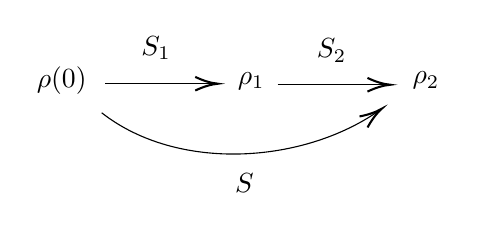
\begin{tikzpicture}[x=0.75pt,y=0.75pt,yscale=-1,xscale=1]
%uncomment if require: \path (0,300); %set diagram left start at 0, and has height of 300

%Straight Lines [id:da4078450591380367] 
\draw    (186,145.5) -- (238.25,145.5) ;
\draw [shift={(240.25,145.5)}, rotate = 180] [color={rgb, 255:red, 0; green, 0; blue, 0 }  ][line width=0.75]    (10.93,-3.29) .. controls (6.95,-1.4) and (3.31,-0.3) .. (0,0) .. controls (3.31,0.3) and (6.95,1.4) .. (10.93,3.29)   ;

%Straight Lines [id:da9736233485654777] 
\draw    (269,146) -- (321.25,146) ;
\draw [shift={(323.25,146)}, rotate = 180] [color={rgb, 255:red, 0; green, 0; blue, 0 }  ][line width=0.75]    (10.93,-3.29) .. controls (6.95,-1.4) and (3.31,-0.3) .. (0,0) .. controls (3.31,0.3) and (6.95,1.4) .. (10.93,3.29)   ;

%Curve Lines [id:da5450320200035714] 
\draw    (184.25,159.5) .. controls (220.88,188.21) and (281.52,184.09) .. (318.15,158.29) ;
\draw [shift={(319.25,157.5)}, rotate = 504.02] [color={rgb, 255:red, 0; green, 0; blue, 0 }  ][line width=0.75]    (10.93,-3.29) .. controls (6.95,-1.4) and (3.31,-0.3) .. (0,0) .. controls (3.31,0.3) and (6.95,1.4) .. (10.93,3.29)   ;


% Text Node
\draw (165,143.83) node   {$\rho ( 0)$};
% Text Node
\draw (256.33,144.17) node   {$\rho _{1}$};
% Text Node
\draw (340.5,144) node   {$\rho _{2}$};
% Text Node
\draw (253,193.5) node   {$S$};
% Text Node
\draw (210.5,128.5) node   {$S_{1}$};
% Text Node
\draw (295,129.5) node   {$S_{2}$};


\end{tikzpicture}
\end{center}

e il risultato è ancora una mappa di Kraus $S(\rho) = (S_2 \circ S_1)(\rho) = S_2(S_1(\rho))$ che gode ancora di tutte le proprietà di $S$.
\item \textbf{Invertibilità}. Data $S$, $S^{-1}$ esiste solo se è anche unitaria. Se non lo è significa, fisicamente, che vi è stata un'interazione tra $A$ e $B$ che non è racchiusa nella descrizione di $A$ data da $\rho_A$, cioè si è persa dell'informazione nel passaggio da $\rho_{A+B}$ alla singola $\rho_A$.
\end{itemize}

\subsection{Krauss Representation Theorem}
L'aver elencato le proprietà di $S$ ci permette di \textbf{generalizzare} tale costruzione.\\
Data infatti una mappa \textit{tra stati} $S: \rho_1 \to \rho_1'$ (detta anche \textit{superoperatore}, dato che è un operatore che agisce su una matrice - cioè su un'osservabile) con le seguenti proprietà:
\begin{enumerate}
\item Lineare
\item Manda matrici Hermitiane in matrici Hermitiane
\item Conserva la traccia
\item Completamente positiva
\end{enumerate}
Allora $S$ si può scrivere in \textbf{rappresentazione di Kraus}, cioè nella forma \q{decomposta}:
\begin{align*}
\rho_1' = \sum_{k=1}^{\op{dim}\hs_2} E_k \rho_1 E_k^\dag \qquad \sum_{k}E_k^\dag E_k = 1
\end{align*}

\textbf{Nota}: in questa formula generale, \textbf{non} è richiesto che $\rho_1$ derivi da una $\rho_{12}$ composta separabile.

\subsubsection{Esempio}
Sia $\rho_1$ la matrice densità di un generico qubit. Consideriamo il sistema di $2$ qubit nello stato $\rho$ \textbf{separabile}:
\begin{align*}
\rho = \begin{pmatrix} \rho_1 & 0 \\ 0 & 0\end{pmatrix} = \begin{pmatrix}1 & 0\\ 0 & 0 \end{pmatrix} \otimes \rho_1 = \ket{0}_2\bra{0}_2 \otimes \rho_1
\end{align*}

Facciamo evolvere unitariamente la $\rho$, ed esaminiamo quanto accade per $\rho_1$:
\begin{align*}
\rho_1' = \underset{2}{\op{Tr}}(U\rho U^\dag) \underset{(a)}{=} \underset{2}{\op{Tr}} \left(\begin{pmatrix}A & B\\ C & D \end{pmatrix} \begin{pmatrix} \rho_1 & 0\\ 0 & 0 \end{pmatrix}\begin{pmatrix} A^\dag & C^\dag\\ B^\dag & D^\dag \end{pmatrix}\right) = A \rho_1 A^\dag + C \rho_1 C^\dag
\end{align*}
dove in (a) rappresentiamo le matrici $U$ e $U^\dag$ in una forma a blocchi $2\times 2$.\\

Confrontando con la formula generale in (\ref{eqn:kraus-rep}), troviamo che $E_k = \{A,C\}$.\\
Verifichiamo che la traccia è conservata:
\begin{align*}
\op{Tr}(\rho_1') &= \op{Tr}(A\rho_1 A^\dag + C\rho_1 C^\dag) \underset{(a)}{=} \op{Tr}(\rho_1 A A^\dag) + \op{Tr}(\rho_1 CC^\dag) =\\
&= \op{Tr}(\rho(\underbrace{AA^\dag + CC^\dag}_{\bb{I}})) = \op{Tr}(\rho_1)
\end{align*}
dove in (a) abbiamo usato la ciclicità della traccia, cioè l'invarianza per permutazione cicliche dell'argomento:
\begin{align*}
\op{Tr}(ABC)=\op{Tr}(BCA) = \op{Tr}(CAB)
\end{align*}

\begin{comment}
Con operazioni di questo tipo possiamo esplorare stati \q{all'interno} della sfera di Bloch, considerando quindi un'evoluzione non unitaria, dato che si perde la reversibilità. Per esempio, l'origine della sfera di Bloch corrisponde allo stato massimamente misto, e chiaramente un'evoluzione che porta dalla superficie della sfera di Bloch all'origine non può essere reversibile, dato che l'informazione del punto di partenza viene persa nel tragitto.


\end{comment}

\end{document}

